\section{Numerical Experiments}
As the final part of our report, we implement the algorithms in the original article with \texttt{Julia} and its package \texttt{DifferentialEquations.jl} \cite{rackauckas2017differentialequations}. By comparing ODE direct discretizating (DD) methods described in the article against gradient descent (GD) and Nesterov's accelerated gradient (NAG) methods, we con verify the main results in the theoretical part. The code of these experiments can be found here: \url{https://github.com/xiaoxuan-yu/Direct-Runge-Kutta-Discretization-Achieves-Acceleration-PKU}.

Inspired by the numerical results by \textcite{NEURIPS2019_7a2b33c6}, we generate normal distributed separable dataset and fit a linear model \(Ax=b\). Then, we minimize three different kinds of loss functions:
\begin{equation}
    \begin{aligned}
        f_1(x) & = \left\| Ax-b \right\|_{2}^2                \\
        f_2(x) & = \sum_{i}\log(1+e^{-w_i^{\mathrm{T}}x y_i}) \\
        f_3(x) & = \frac{1}{4}\left\| Ax-b \right\|_{4}^4
    \end{aligned}
\end{equation}
where $f_1(\cdot ),f_2(\cdot ),f_3(\cdot )$ are $L_2$ loss, logistic loss and $L_4$ loss, respectively. For each test case and optimization algorithm, we empirically select the learning rate as the largest step length among $\{ 10^{-k}|k\in \mathbb{Z} \}$ that the method remains stable during the optimization process. Main results are shown in Figure \ref{Numerical} where all figures are on log-log scale.
\begin{figure}[htbp]
    \begin{subfigure}{0.45\textwidth}
        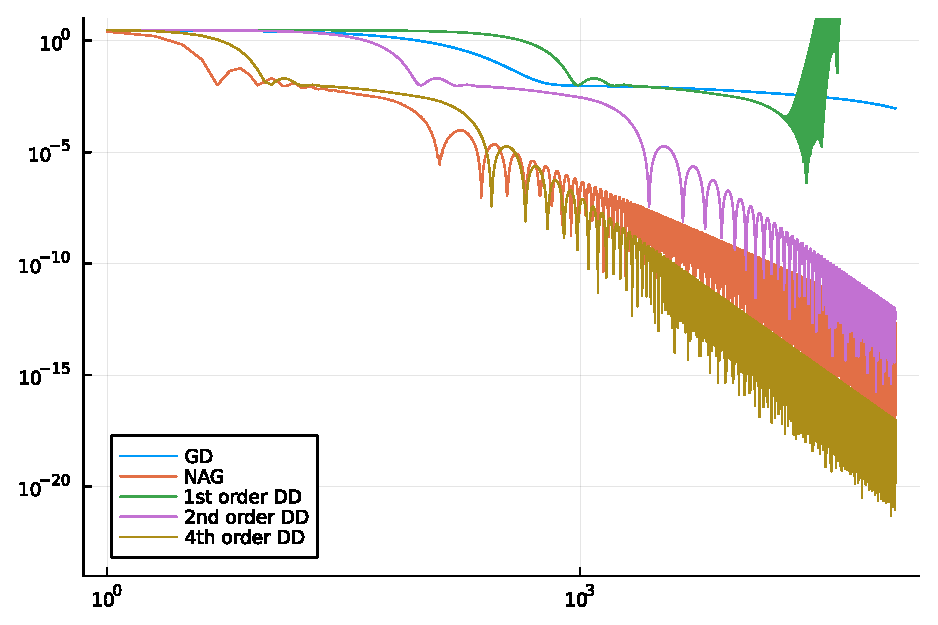
\includegraphics[width=\textwidth]{"assets/quadratic-1.pdf"}
        \caption{}
        \label{fig:l2-1}
    \end{subfigure}
    \hfill
    \begin{subfigure}{0.45\textwidth}
        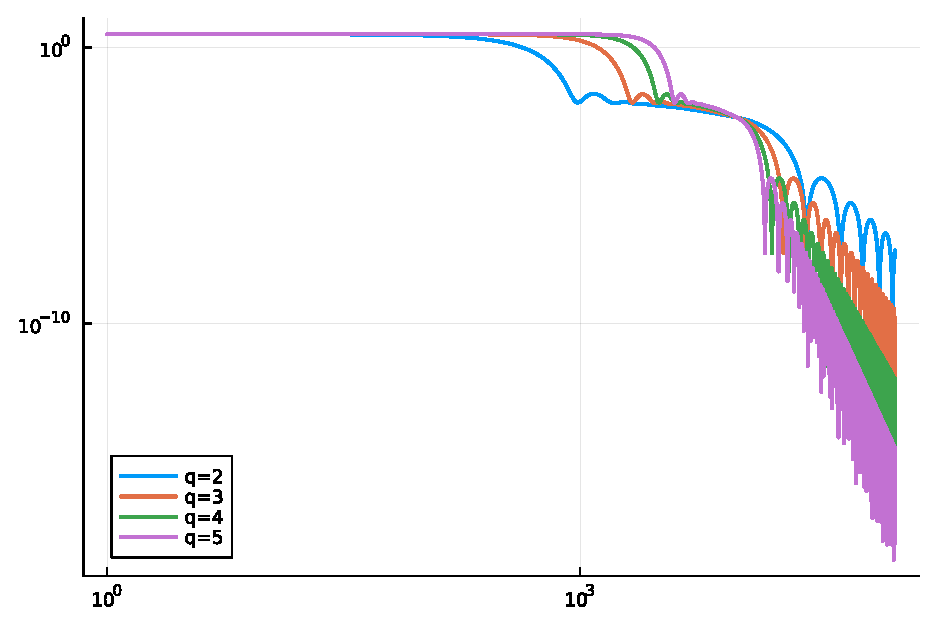
\includegraphics[width=\textwidth]{"assets/quadratic-2.pdf"}
        \caption{}
        \label{fig:l2-2}
    \end{subfigure}
    \hfill
    \begin{subfigure}{0.45\textwidth}
        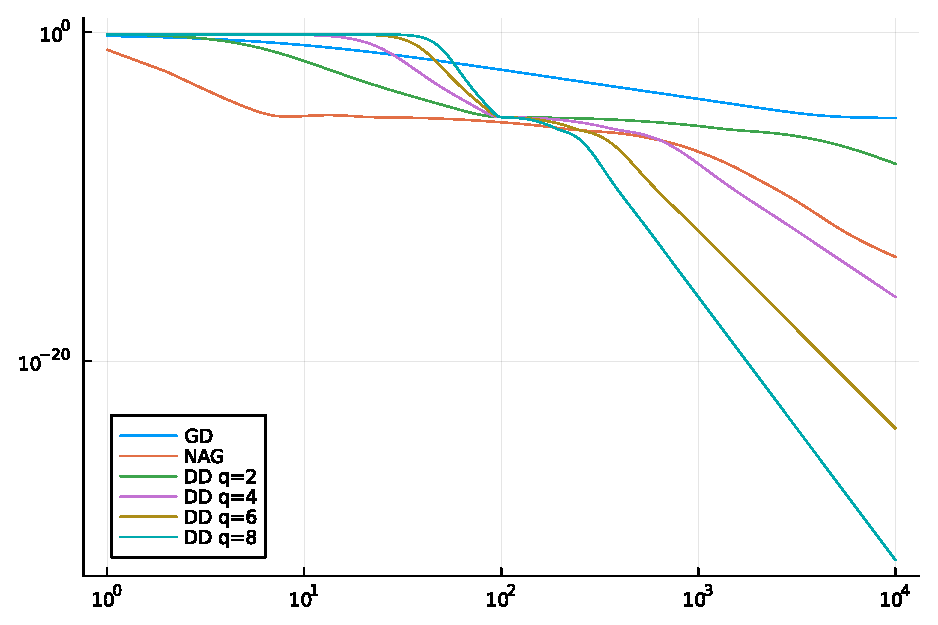
\includegraphics[width=\textwidth]{"assets/l4loss.pdf"}
        \caption{}
        \label{l4}
    \end{subfigure}
    \hfill
    \begin{subfigure}{0.45\textwidth}
        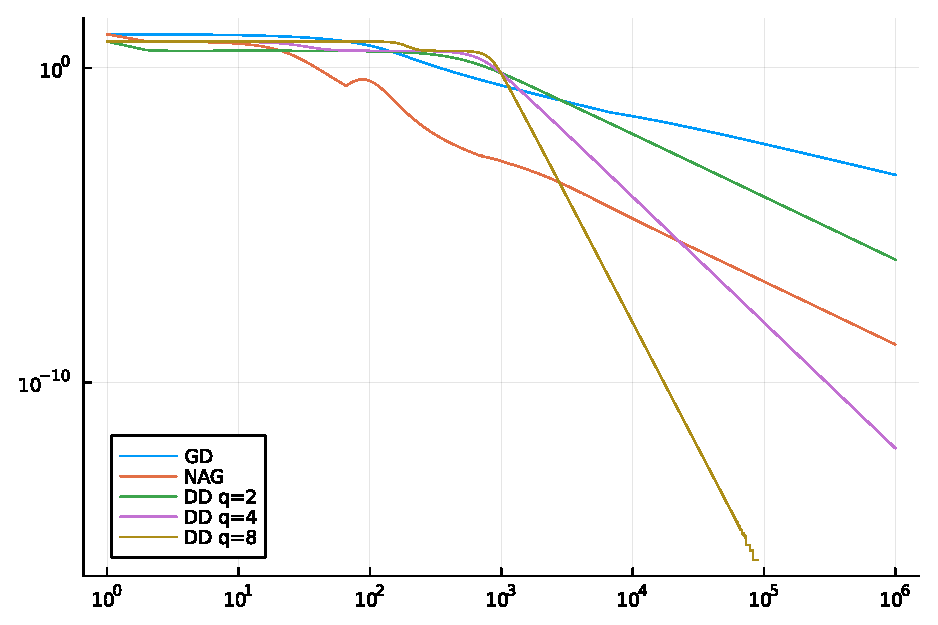
\includegraphics[width=\textwidth]{"assets/logistic.pdf"}
        \caption{}
        \label{fig:logistic}
    \end{subfigure}
    \caption{Experimental results comparing DD with GD and NAG. (a) Convergence path of GD, NAG and DD with different Runge-Kutta integrators of degree $s=1, 2, 4$ on $L_2$ loss. (b) The optimization of $L_2$ loss by DD with different choices of $q$ values with 4-th order Runge-Kutta integrator RK4. (c) Minimization of $L_4$ loss by GD, NAG and DD with different $q$ vaues with a 2-nd order Runge-Kutta integrator. (d) Minimization of logistic loss by GD, NAG and DD with different $q$ vaues with a 4-th order Runge-Kutta integrator.}
    \label{Numerical}
\end{figure}

First, we explore the optimization path of a quadratic function, the $L_2$ loss, w.r.t. iteration. In particular, we labeled half of the generated data by 0 and the rest by 1. In Figure \ref{fig:l2-1}, the ODE is discretized for $p=2$ with different Runge-Kutta integrators with $s \in \{ 1,2,4 \}$ and compared against GD and NAG algorithm. We can find that except the integrator with $s=1$ can not converge due to the unstability of the differential format itself, the DD methods shows superiority over GD. By using higher order iterator, the local acceleration is achieved and 4th order DD even converges faster than NAG (although for each iteration, it is obviously more costly than NAG). In Figure \ref{fig:l2-2}, we explore the effect of $q$ is the ODE. Since in the article $p$ keeps the same as the one in the assumption, thus we denotes $q$ the true parameter used in the ODE as below
$$
    \ddot x(t) + \frac{2q+1}{t}\dot x(t)+q^2 t^{q-2}\nabla  f(x(t)) = 0.
$$
We optimize the same $L_2$ loss with different values of $q$. By selecting smaller learning rates and increasing the numerical precision by using longer floats, the phenomenon that DD method diverges when $q>2$ is not observed. Instead, we found that for $q \in \{ 2,3,4,5 \}$, larger $q$ will give out faster convergence.

Then the minimization of $L_4$ loss (Figure \ref{l4}) and logistic loss (Figure \ref{fig:logistic}) is studied. We use 2-nd order Runge-Kutta integrator SSPRK22 for logistic loss optimization and 4-th order Runge-Kutta integrator RK4 for $L_4$ loss. As shown in Figure \ref{l4} and \ref{fig:logistic}, the loss decrease faster for larger $q$, as we can observed in above experiment about $L_2$ loss.